
\documentclass[t, 11pt]{beamer}
\pdfmapfile{+sansmathaccent.map}
%%% Работа с русским языком
\usepackage{cmap}				
\usepackage{mathtext} 				
\usepackage[T2A]{fontenc}		
\usepackage[utf8]{inputenc}			
\usepackage[russian, english]{babel}	

\usetheme{Montpellier}
\usecolortheme{beaver} % Цветовая схема



%%% Работа с картинками
\usepackage{graphicx}

\usepackage{csquotes}

\hypersetup{				
	colorlinks=true,       	
	linkcolor=blue,          
	citecolor=black,       
	filecolor=magenta,      
	urlcolor=red           
}
%% табличка
\usepackage{booktabs, caption, makecell}
\usepackage{threeparttable}

%% график нормального распределения 
\usepackage{tikz}
\usepackage{xcolor}
\usepackage{pgfplots}
\pgfplotsset{compat=1.7}

%% доп символы
\usepackage{newunicodechar}

\newcommand\Warning{%
	\makebox[1.4em][c]{%
		\makebox[0pt][c]{\raisebox{.1em}{\small!}}%
		\makebox[0pt][c]{\color{red}\Large$\bigtriangleup$}}}%

\newunicodechar{⚠}{\Warning}

\title {Statistical tests}
\subtitle{Intro to Statistical Inference Part 2}
\author{Chuvakin Sergey}
\date{\today}
\institute[<<Anthropology>>]{<<School of Advanced Studies>>}

\begin{document}

	
	\frame[plain]{\titlepage}		
	
	\section{Outline}
	
		\begin{frame} 
			\frametitle{\insertsection} 
			\begin{itemize}
				\item Compare more than two groups
				\item Chi-squared test
				\item Correlations
			\end{itemize}
		\end{frame}
		
	\section{Compare more than two groups}
	
	\subsection{ANOVA}
	\begin{frame} 
		\frametitle{\insertsection} 
		ANOVA - ANalysis Of VAriance - statistics that help to point out the difference between two or more groups. Detailed information \href{https://www.statsdirect.com/help/analysis_of_variance/one_way.htm} {here}
		
		\vspace{1cm}
		
		\Warning Variances of groups should be homogenious
		
		\Warning The post hoc test is required


	\end{frame}

	\subsection{Post hoc test}
\begin{frame} 
	\frametitle{\insertsection} 	
	
	Post hos test - is a test that usually conducted after analysis (<<post hoc>>), to precise inferences. I.e. it could be box plots! 
	
	\begin{center}
		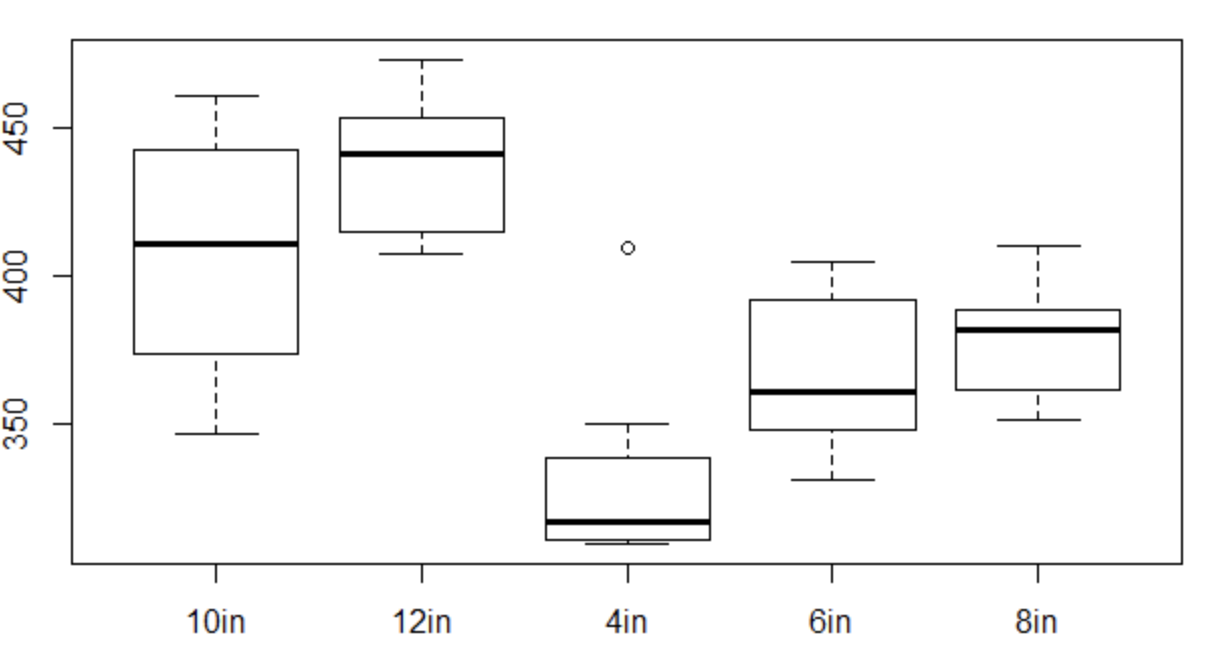
\includegraphics[scale=0.4]{post-hoc}
	\end{center}
	
\end{frame}
	\section{Chi-Square test}
			\begin{frame} 
		\frametitle{\insertsection} 
		$\chi^2$ - Popular statistics to test if matrix has non uniform distribution. It return Chi square that can be easily transformed to P-value. 
		
		Let's use example for explanation!
		
		\vspace{1cm}
		
		H0 - Gender and preference for cats or dogs are independent.
		
		H1 - Gender and preference for cats or dogs are not independent.
		
		
	\end{frame}

\begin{frame} 
	\frametitle{\insertsection} 	
	
	\begin{center}
		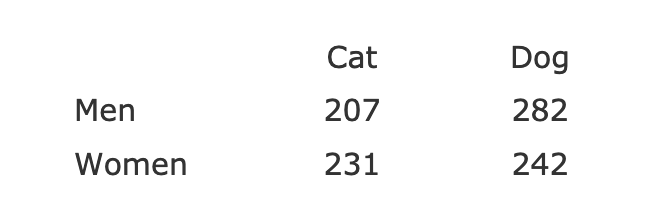
\includegraphics[scale=0.7]{chi1}
	\end{center}
	
\end{frame}

\begin{frame} 
	\frametitle{\insertsection} 	
	
	\begin{center}
		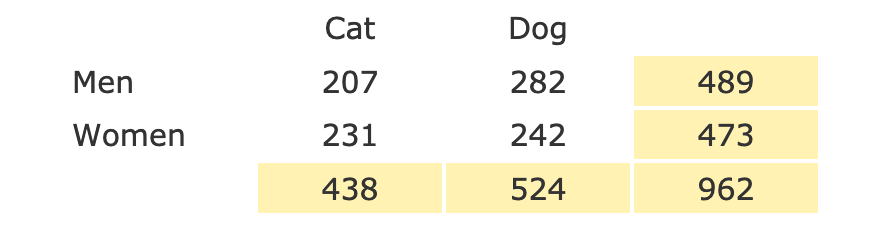
\includegraphics[scale=0.7]{chi2}
	\end{center}
	
\end{frame}

	\begin{frame} 
		\frametitle{\insertsection} 	
		
		\begin{center}
			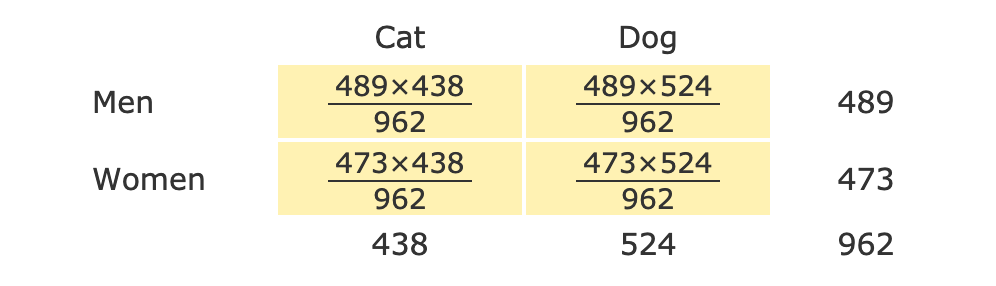
\includegraphics[scale=0.7]{chi3}
		\end{center}
		
	\end{frame}
	
	\begin{frame} 
		\frametitle{\insertsection} 	
		
		\begin{center}
			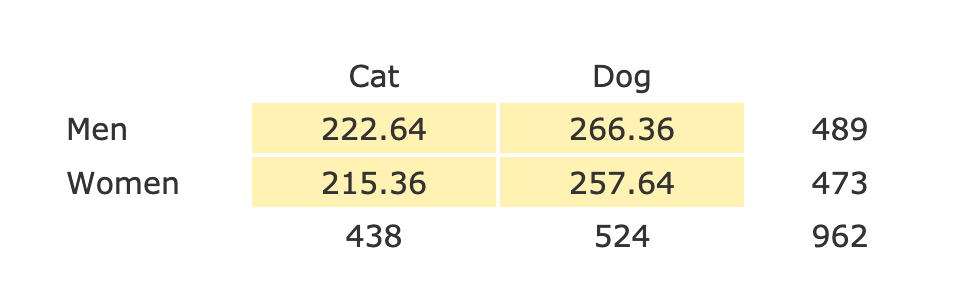
\includegraphics[scale=0.7]{chi4}
		\end{center}
		
	\end{frame}

		\begin{frame} 
	\frametitle{\insertsection} 	

Subtract expected from observed, square it, then divide by expected:

In other words, use formula 

$$\frac{(O - E)^2}{E}$$

where:

\vspace{1cm}

O = Observed (actual) value

E = Expected value

	
\end{frame}
	
		\begin{frame} 
		\frametitle{\insertsection} 	
		
		\begin{center}
			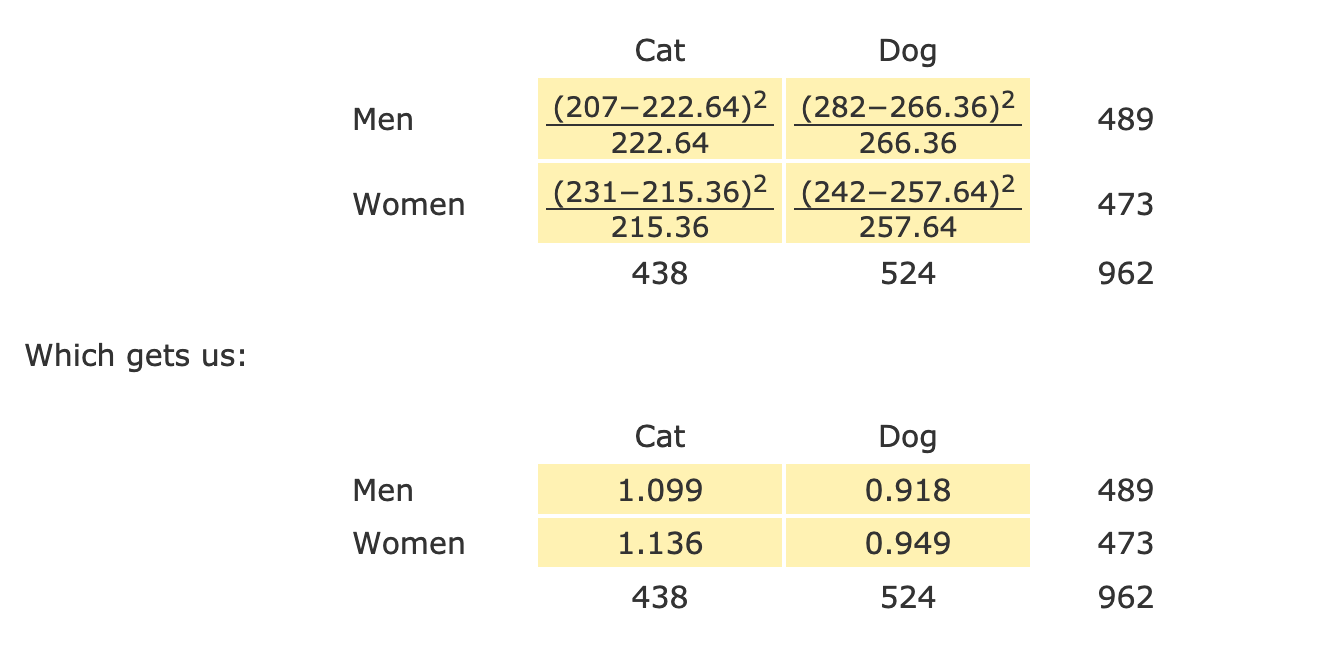
\includegraphics[scale=0.5]{chi5big}
		\end{center}
		
	\end{frame}

		\begin{frame} 
	\frametitle{\insertsection} 	
	
	Now add up those calculated values:
	
	1.099 + 0.918 + 1.136 + 0.949 = 4.102
	
	\emph{Chi-Square} is 4.102

	Than look into table \href{https://www.mathsisfun.com/data/chi-square-table.html}{here}.
	
	Make inference!
	\end{frame}
	
\section{Correlation}	

			\begin{frame} 
		\frametitle{\insertsection} 	
		Correlation - is the most popular way to answer the question: what is the relation between two variables. It returns metrics between 0 and 1 that shows how two vector move together. It's standartized version of covariance
		
		\begin{itemize}
			\item Reference point: cov x,y=0 means X and Y have nothing incommon
			\item Positive covariance values indicate positive association: the bigger X the bigger Y 
			\item Negative covariance values indicate negative association: thebigger X the smaller Y
		\end{itemize}

	\end{frame}
	
				\begin{frame} 
		\frametitle{\insertsection} 	
	 One of the assumtions of correlation is  - variables whould be measured in one space. For example we can compare number of death per capita and per 100 000. 
	 
	 \vspace{0.5cm}
	 
	 Standardization is a general method of transforming inputvariables (e.g. X or Y) or some statistical measures of interest(e.g. covariance coefficient) in a way that eliminates scale effects.
	 	 
	 \vspace{0.5cm}
	 
	 E.g., standardizing a normally distributed variable means converting it to the standard normal distribution (with zero mean and unit standard deviation). After standardization, this variable is no longer measured in meters, years, or dollars, but in standard deviations
	 
	\end{frame}

				\begin{frame} 
	\frametitle{\insertsection} 	
		Generic standardization formula (Z-score formula):
		$$z_i = \frac{x_i- \hat{x}}{\sigma_x}$$
		Covariance
		$$Cov(X,Y) = E[(X-\mu_x)(Y-\mu_y)]$$
		Correlation
		$$r = \frac{cov_{x,y}}{\sigma_x \times \sigma_y}$$
	
\end{frame}
	


\subsection{Assumptions}


\begin{frame} 
	\frametitle{\insertsection} 	
	\framesubtitle{\insertsubsection} 	
	
	\begin{itemize}
		\item Continious variables
		\item Normal distribution
		\end{itemize}
	
\end{frame}

\begin{frame} 
	\frametitle{\insertsection} 	
	\framesubtitle{\insertsubsection} 	
	
Otherwise use non-parametric alternatives!
\begin{itemize}
	\item Spearman’s $\rho$ (also reads as rho)
	
 \item 	Kendall’s $\tau$ (reads as tau)
	
 \item 	Interpretation is pretty much the same as with Pearson’s r:same effect size cut-offs, same p-value thresholds
	
	\item Use the method = argument of cor() or cor.test to choose a relevant correlation coefficient (three options: pearson(default), spearman, and kendall, all should be typed inlower case)
\end{itemize}


\end{frame}
\end{document}